%
% CHAPTER - Philosophy of Science
%

\chapterimage{LHC.pdf} % Chapter heading image

\chapter{Philosophy of Science}
\label{chap:philosophy-science}

\begin{quote}
\begin{flushright}
\emph{Science may be regarded as the art of data compression.}\\
Li \& Vitányi
\end{flushright}
\end{quote}
\bigskip

%
% Section: Wikipedia, The Free Encyclopedia
%

\section{Wikipedia, The Free Encyclopedia}

the analyses performed will be based on the collection of scientific pages from Wikipedia. As we will see, Wikipedia pages not only contain the encyclopedic coverage of research topics that we need for the theory of nesciece, they are also a highly cited reference in the scientific community, and they are very well known by the general public. These two additional characteristics make this collection of articles a highly valuable resource to validate our methodology in practice.



Wikipedia pages are written in the \emph{MediaWiki Markup Language}, which provides a simple notation for formatting text, so that users without knowledge of XHTML or CSS can edit them easily. MediaWiki tags are often misused by editors, therefore it is required to apply several heuristics in order to circumvent those problems. We have used an advanced \emph{Wikipedia Extractor} utility to extract the relevant text of the pages. Also the extractor was instructed to remove all those non relevant elements for our analysis, such as images, tables, references and lists. 

%
% Section: Classification of Research Topics
%

\section{Classification of Research Topics}
\label{sec:Classification_Research_Topics}

{\color{red} TODO: Talk about compressors, its behavior depending of size of object and window (buffer) size, and the speed-compression ratio trade off.}

The Kolmogorov complexity of a page was estimated using the compressed
version of the text. As compressed tool we have used the Unix \texttt{gzip}
utility, that it is based on a combination of the Lempel-Ziv LZ77
algorithm and Huffman coding. Figure \ref{fig:Nescience-of-Topics}
shows a plot of nescience for all the topics after normalization.

\begin{figure}[h]
\centering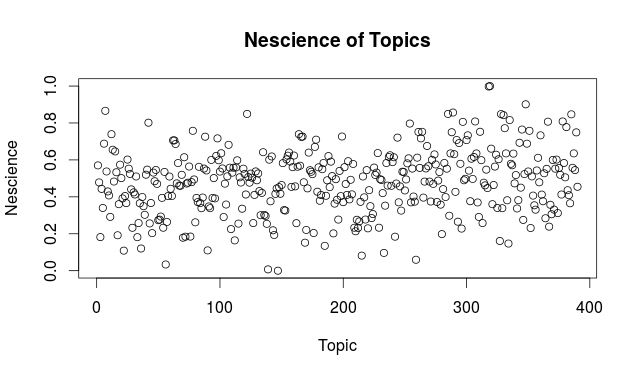
\includegraphics[scale=0.5]{NescienceTopics}
\caption{\label{fig:Nescience-of-Topics}Nescience of topics}
\end{figure}

Table \ref{tab:Nescience-of-topics} contain the ten topics with highest
nescience, and the normalized version of this number. The identification
of the topics with highest nescience is even more controversial. Some
authors would argue that the topics listed in the table are the least
known topics in the area of theory of computation, like for example
\emph{UML state machine} or \emph{Kleene's recursion theorem}. However
the list includes very difficult to address topics, \emph{computability}
and \emph{computability theory}, and hot research topics like the
\emph{Kolmogorov structure function}. It is also remarkable that the
list contains three related topics, \emph{analytical hierarchy}, \emph{arithmetical
hierarchy} and \emph{hyperarithmetical theory}, suggesting that this
is a highly unknown area of knowledge. An important point to mention
is that our computed nescience is not directly proportional to the
length of the article, and so, the list of the topics with the higher
nescience does not mimic the list of the lengthiest articles.

\begin{table}
\begin{centering}
\begin{tabular}{|c|c|c|}
\hline 
Topic & Nescience & Norm.\tabularnewline
\hline 
\hline 
Arithmetical hierarchy & 2.28 & 1.00\tabularnewline
\hline 
Analytical hierarchy & 2.28 & 1.00\tabularnewline
\hline 
Hyperarithmetical theory & 2.13 & 0.90\tabularnewline
\hline 
Kolmogorov struct. funct. & 2.08 & 0.87\tabularnewline
\hline 
Behavior of DEVS & 2.06 & 0.86\tabularnewline
\hline 
UML state machine & 2.05 & 0.85\tabularnewline
\hline 
Computability & 2.05 & 0.85\tabularnewline
\hline 
Kleene's recursion th. & 2.05 & 0.85\tabularnewline
\hline 
Computability theory & 2.04 & 0.84\tabularnewline
\hline 
Computation in the limit & 2.00 & 0.82\tabularnewline
\hline 
\end{tabular}
\par\end{centering}

\caption{\label{tab:Nescience-of-topics}Nescience of topics}
\end{table}


In practice, our definition of nescience is problematic when we work
with very short descriptions, since the compressed version of the
text could be larger than the uncompressed version, given an negative
nescience. This is still an open problem that must be addressed, perhaps
by borrowing some techniques from the minimum description length principle.

The maturity of a topic is estimated based on the length of the Wikipedia
article (only the text), and the length of the compressed version.
Figure \ref{fig:Maturity-of-Topics} shows a plot of the maturity
of the selected set of topics after the normalization process.

\begin{figure}[h]
\centering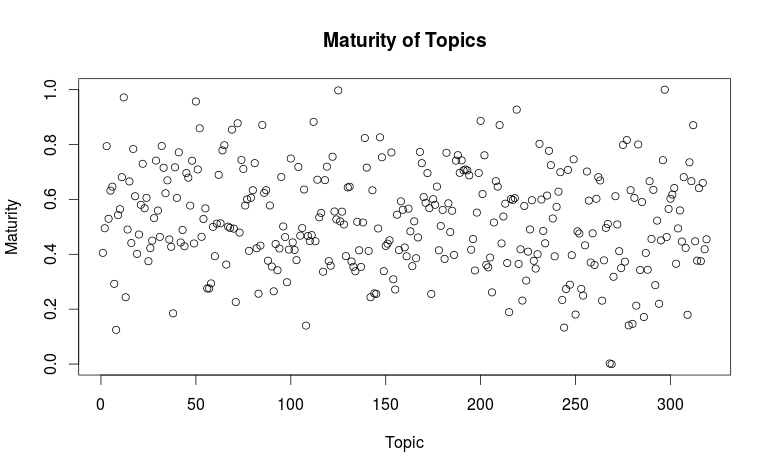
\includegraphics[scale=0.5]{MaturityTopics}
\caption{\label{fig:Maturity-of-Topics}Maturity of topics}
\end{figure}

Table \ref{tab:Maturity-of-Topics} contains the ten most relevant
topics according to its maturity. For each topic it is shown the maturity
and the normalized version of this number. Well classified topics,
that is, topics that our intuition tell us that are well understood,
could include \emph{Read-only right moving Turing machines}, \emph{Crossing
sequence (Turing machines)}, and perhaps the \emph{P'' language}.
Other topics that perhaps are misclassified include \emph{communication
X-Machine}, \emph{Power DEVS}, \emph{MIPR}, and \emph{constraint automaton}.

\begin{table}
\begin{centering}
\begin{tabular}{|c|c|c|}
\hline 
Topic & Maturity & Norm.\tabularnewline
\hline 
\hline 
Carry operator & 5.34 & 1.00\tabularnewline
\hline 
Binade & 4.54 & 0.99\tabularnewline
\hline 
Comm. X-Machine & 3.01 & 0.97\tabularnewline
\hline 
PowerDEVS & 2.35 & 0.94\tabularnewline
\hline 
MPIR & 2.00 & 0.92\tabularnewline
\hline 
Constraint automaton & 1.84 & 0.90\tabularnewline
\hline 
RO right moving TM & 1.73 & 0.89\tabularnewline
\hline 
P'' & 1.71 & 0.89\tabularnewline
\hline 
Crossing sequence (TM) & 1.63 & 0.88\tabularnewline
\hline 
Microsoft Binary Format & 1.53 & 0.86\tabularnewline
\hline 
\end{tabular}
\par\end{centering}

\caption{\label{tab:Maturity-of-Topics}Maturity of topics}
\end{table}


The most difficult part of the identification of topics as tools,
that is, topics with very high maturity (or very low nescience), is
to distinguish when the description of a topic is short because it
is well understood (for example, a mathematical theorem), or when
it is short because it is a unfinished or poorly written article.
Our work is based on the classification of Wikipedia articles as stubs,
however, this classification is not very reliable, since many stubs
articles are not classified as such (many of the misclassified topics
suffer from this problem). How to automatically distinguish between
a well-understood topic and a poorly written description is still
an open question.

The interest of a topic as a tool measures how likely is that this
tool can be applied to other problems. Figure \ref{fig:Interestingness-of-Tools}
shows a plot of the interestingness of the selected set of topics
after the normalization process.

\begin{figure}[h]
\centering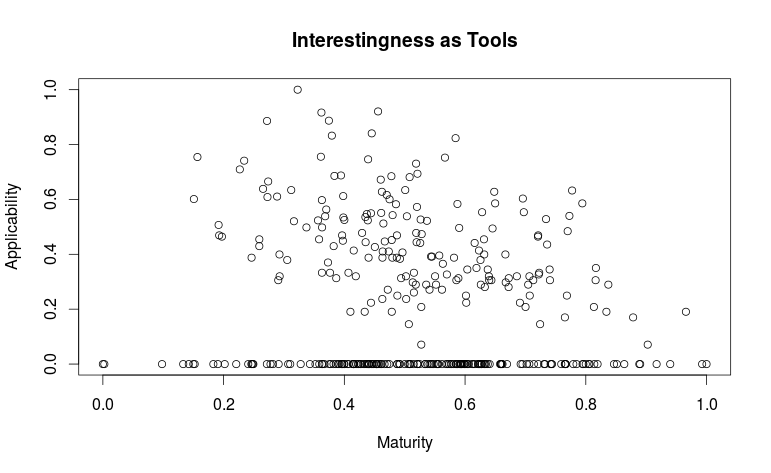
\includegraphics[scale=0.5]{InterestingnessTools}
\caption{\label{fig:Interestingness-of-Tools}Interestingness of Tools}
\end{figure}

Table \ref{tab:Interestingness-of-Tools} contains the ten most relevant
topics according to its interestingness as a source of interesting
tools. Out of the ten topics, only two (\emph{ternary numeral system}
and \emph{recursion}) appear in the list of top ten mature topics
or top ten applicable topics; the rest of topics are new. In the list
we can find topics like the \emph{GNU Multiple Precision Arithmetic
Library} and the \emph{standard for radix-independent floating-point
arithmetic} (IEEE 854-1987) that are definitely tools, but not in
the sense of tool that we are looking for our methodology. Some other
topics are not clear that can be considered as tools, like \emph{arithmetic
logic unit}, \emph{barrel shifter}, or \emph{arithmetic overflow}.
Topics that match or intuitive idea of tool include \emph{recursion},
\emph{state space}, \emph{abstract machine}, and \emph{ternary numeral
system}. There are also some topics, like \emph{computational model},
too broad to be considered in a question.

\begin{table}
\begin{centering}
\begin{tabular}{|c|c|}
\hline 
Topic & Interestingness\tabularnewline
\hline 
\hline 
GNU MPAL & 0.49\tabularnewline
\hline 
Ternary numeral system & 0.48\tabularnewline
\hline 
IEEE 854-1987 & 0.47\tabularnewline
\hline 
Arithmetic logic unit & 0.43\tabularnewline
\hline 
Recursion & 0.42\tabularnewline
\hline 
Barrel shifter & 0.42\tabularnewline
\hline 
State space & 0.42\tabularnewline
\hline 
Abstract machine & 0.41\tabularnewline
\hline 
Computational model & 0.39\tabularnewline
\hline 
Arithmetic overflow & 0.39\tabularnewline
\hline 
\end{tabular}
\par\end{centering}

\caption{\label{tab:Interestingness-of-Tools}Interestingness of Tools}
\end{table}

Finally, Figure \ref{fig:Interestingness-of-Questions} contains a
plot of the interestingness of the topics considered as potential
interesting problems.

\begin{figure}[h]
\centering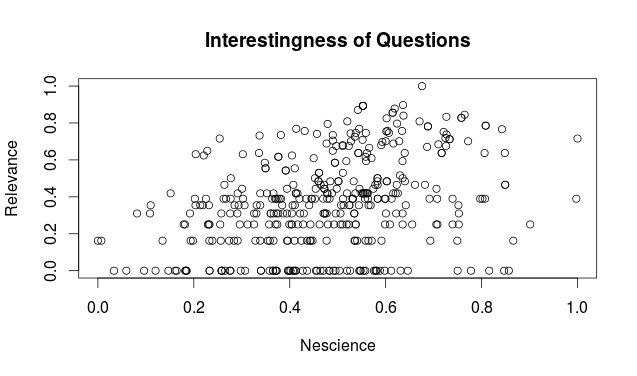
\includegraphics[scale=0.5]{InterestingnessQuestions}
\caption{\label{fig:Interestingness-of-Questions}Interestingness of Questions}
\end{figure}

Table \ref{tab:Interestingness-of-Problems} shows the ten most interesting
topics as interesting problems. Topics that fit our intuitive idea
of problem, that is, not very well understood concepts with a high
relevance, could include \emph{arithmetical theory}, \emph{halting
problem}, \emph{floating point}, \emph{quantum computer}, and \emph{computable
function}. The topic \emph{recursion} appears both as a tool and as
a problem. However in case of tools it refers to the concept of recursion
in general, and in case of problems it refers to the implementation
of the concept of recursion in the particular case of computer science.
The case of \emph{regular expression}, a topic that intuitively should
be classified as a tool and not as a problem, can be explained due
to the length of the article in Wikipedia, that provides a detailed
description of the language used for regular expressions. This problem
rises the question of how to distinguish in Wikipedia between introductory
articles and reference articles. Finally, there are topics like \emph{computability
theory}, \emph{lambda calculus} and \emph{computability} that are
too broad to be analyzed as problems.

\begin{table}
\begin{centering}
\begin{tabular}{|c|c|}
\hline 
Topic & Interestingness\tabularnewline
\hline 
\hline 
Arithmetical hierarchy & 0.72\tabularnewline
\hline 
Regular expression & 0.68\tabularnewline
\hline 
Computability theory & 0.65\tabularnewline
\hline 
Halting problem & 0.65\tabularnewline
\hline 
Recursion (CS) & 0.64\tabularnewline
\hline 
Lambda calculus & 0.63\tabularnewline
\hline 
Floating point & 0.61\tabularnewline
\hline 
Quantum computer & 0.57\tabularnewline
\hline 
Computability & 0.55\tabularnewline
\hline 
Computable function & 0.55\tabularnewline
\hline 
\end{tabular}
\par\end{centering}

\caption{\label{tab:Interestingness-of-Problems}Interestingness of Problems}
\end{table}

\begin{remark}
Based on the given definition of "Interestingness of a topic as a tool", we can explore various mathematical properties and concepts derived from this idea. Some possibilities include:

\begin{itemize}

\item Normalization: To compare different topics fairly, we can normalize their interestingness values by scaling them to a specific range, e.g., [0, 1]. This normalization can help compare the relative interestingness of various topics.

\item Weighted Interestingness: We can introduce weights to the maturity and applicability dimensions to emphasize one over the other depending on the specific context or application. This would allow us to fine-tune the interestingness measure for different scenarios.

\item Correlation: Studying the correlation between maturity and applicability could provide insights into how these dimensions are related and possibly reveal trends across different research topics.

\item Cluster Analysis: By examining topics in the two-dimensional vector space defined by maturity and applicability, we can perform cluster analysis to identify groups of topics with similar levels of interestingness. This can help identify areas of research that share characteristics and possibly suggest interdisciplinary research opportunities.

\item Rate of Change: Investigating the rate of change of interestingness over time can provide insights into the evolving landscape of a research field. This analysis could reveal emerging topics or those that are becoming less relevant.

\item Optimization: Using the interestingness metric, we can explore optimization techniques to find the most interesting topics given certain constraints or within specific domains. This could be useful for research prioritization and resource allocation.

\end{itemize}

These derived mathematical properties and concepts can provide a deeper understanding of the interestingness of research topics and their potential application as tools for solving problems.

\end{remark}

%
% Classification of Resarch Areas
%
\section{Classification of Research Areas}

In this section we analyze the interests of the different research
areas, instead of the interest of individual topics. The areas analyzed
are \emph{sociology} (Level 1 \emph{social sciences}, 6,004 topics),
\emph{biology} (Level 1 \emph{natural sciences}, 6,989 topics), \emph{computer
science} (Level 1 \emph{applied sciences}, 1,331 topics), \emph{epistemology}
(Level 1 \emph{cognitive science}, 4,268 topics), \emph{psychology}
(Level 1 \emph{behavioral science}, 7,905 topics), \emph{chemistry}
(Level 1 \emph{physical sciences}, 11,589 topics), and \emph{mathematics}
(Level 1 \emph{formal sciences}, 4,688 topics).

Table \ref{tab:Interestingness-of-Areas-as-Tools} shows the average
applicability and average maturity of each of the selected areas,
and the average interestingness of each area as a source of interesting
tools. The table largely fits our intuitive idea of which areas are
more important as a source of tools: computer science is the area
of highest interest, and sociology is the area with less interest.
The only extrange elements is that epistemology appears as a source
of very interesting tools, even more interesting, on average, than
topics from mathematics (probably because it contains a large ratio
of poorly written articles).

\begin{table*}
\begin{centering}
\begin{tabular}{|c|c|c|c|}
\hline 
Research Area & Applicability & Maturity & Tools\tabularnewline
\hline 
\hline 
Sociology & $1.00\times10^{-3}$ & $2.93\times10^{-3}$ & $3.09\times10^{-3}$\tabularnewline
\hline 
Biology & $9.20\times10^{-4}$ & $4.65\times10^{-3}$ & $4.74\times10^{-3}$\tabularnewline
\hline 
Chemistry & $3.11\times10^{-3}$ & $5.01\times10^{-3}$ & $5.90\times10^{-3}$\tabularnewline
\hline 
Psychology & $1.14\times10^{-3}$ & $6.91\times10^{-3}$ & $7.00\times10^{-3}$\tabularnewline
\hline 
Mathematics & $9.32\times10^{-3}$ & $9.47\times10^{-3}$ & $1.32\times10^{-2}$\tabularnewline
\hline 
Epistemology & $1.55\times10^{-3}$ & $1.75\times10^{-2}$ & $1.76\times10^{-2}$\tabularnewline
\hline 
Computer\_science & $9.93\times10^{-3}$ & $1.90\times10^{-2}$ & $2.15\times10^{-2}$\tabularnewline
\hline 
\end{tabular}
\par\end{centering}

\caption{\label{tab:Interestingness-of-Areas-as-Tools}Interestingness of Areas
as Tools}
\end{table*}


Finally, Table \ref{tab:Interestingness-of-Areas-as-Problems} shows
the relevance and nescience of the selected areas, and their interest
as a source of interesting problems. Again, the results largely match
our intuitive idea of which areas are less understood: sociology is
the area with the highest number of interesting problems, and mathematics
is the area with the lower number of problems.

\begin{table*}
\begin{centering}
\begin{tabular}{|c|c|c|c|}
\hline 
 & Relevance & Nescience & Problems\tabularnewline
\hline 
\hline 
Mathematics & $4.22\times10^{-2}$ & $3.51\times10^{-1}$ & $3.53\times10^{-1}$\tabularnewline
\hline 
Computer\_science & $2.35\times10^{-2}$ & $4.43\times10^{-1}$ & $4.44\times10^{-1}$\tabularnewline
\hline 
Chemistry & $5.95\times10^{-2}$ & $4.66\times10^{-1}$ & $4.70\times10^{-1}$\tabularnewline
\hline 
Biology & $3.85\times10^{-2}$ & $4.75\times10^{-1}$ & $4.77\times10^{-1}$\tabularnewline
\hline 
Psychology & $5.06\times10^{-2}$ & $5.28\times10^{-1}$ & $5.31\times10^{-1}$\tabularnewline
\hline 
Epistemology & $4.54\times10^{-2}$ & $5.30\times10^{-1}$ & $5.32\times10^{-1}$\tabularnewline
\hline 
Sociology & $4.21\times10^{-2}$ & $5.43\times10^{-1}$ & $5.44\times10^{-1}$\tabularnewline
\hline 
\end{tabular}
\par\end{centering}

\caption{\label{tab:Interestingness-of-Areas-as-Problems}Interestingness of
Areas as Problems}
\end{table*}


%
% Section: Interesting Research Questions
%

\section{Interesting Research Questions}

By combining the elements of Table \ref{tab:Interestingness-of-Tools}
and Table \ref{tab:Interestingness-of-Problems} we could come up
with new interesting ideas of how to apply existing tools to open
problems. As it was said above, the goal of the approach described
in this article is to identify highly potential interesting applications,
but is up to the researcher to decide if certain combination of topics
make sense or not, and if they deserve the effort to pursuit them.
The results of the combination is in Table \ref{tab:Interesting-Intradisciplinary-Questions}.

\begin{table*}
\begin{centering}
\begin{tabular}{|l|c|c|}
\hline 
{Tool} & Problem & Interestingness\tabularnewline
\hline 
\hline 
Ternary numeral system & Regular expression & 1.21\tabularnewline
\hline 
{GNU MPAL} & Arithmetical hierarchy & 1.19\tabularnewline
\hline 
IEEE 854-1987 & Arithmetical hierarchy & 1.17\tabularnewline
\hline 
Quantum computer & Regular expression & 1.17\tabularnewline
\hline 
Ternary numeral system & Arithmetical hierarchy & 1.15\tabularnewline
\hline 
Division by zero & Regular expression & 1.15\tabularnewline
\hline 
Turing machine & Regular expression & 1.14\tabularnewline
\hline 
GNU MPAL & Regular expression & 1.13\tabularnewline
\hline 
Ternary numeral system & Halting problem & 1.13\tabularnewline
\hline 
Recursion & Halting\_problem & 1.13\tabularnewline
\hline 
\end{tabular}
\par\end{centering}

\caption{\label{tab:Interesting-Intradisciplinary-Questions}Interesting Intradisciplinary
Questions}
\end{table*}

Most of the interesting questions identified have very low quality.
As it was said before, the problem is that it is very difficult to
distinguish (automatically and unsupervised) between a poorly written
article from a very well understood topic. In this section we review
some on the interesting intradisciplinary questions identified with
the aim to clarify what we mean as interesting question and how interesting
questions should be interpreted. Some combinations worth examining
could be:
\begin{itemize}
\item Interesting Question 7: \emph{Can we apply }Turing machines\emph{
to }regular expressions\emph{?} The answer to this question is yes,
since it is a very well know question. Regular expressions are recognized
by finite automata, and finite automata can be simulated by Turing
machines.
\item Interesting Question 10: \emph{Can we apply }recursion\emph{ to the
}halting problem\emph{?} Again the answer is yes, since the proof
of the halting problem is based on a machine that call itself.
\end{itemize}
Note that both questions have well known answers, and so, we have
failed to provide original questions.

The most interesting questions arise when we combine topics from two
different disciplines. However, the probability that the identified
questions are meaningful is lower than in the case of intradisciplinary
analysis.

For the interdisciplinary analysis we have used the collection of
pages from the theory of computation already used in the intradisciplinary
analysis, and a new collection of topics from the area of\emph{ }bioinformatics.
The topics were selected using the Wikipedia category \emph{natural
sciences}, \emph{biology}, \emph{bio}logical\emph{ processes}. In
total, there were more than $10^{5}$ combinations analyzed. Table
\ref{tab:Interesting-Intradisciplinary-Questions-1-1} contains the
list of the most relevant intradisciplinary applications.

\begin{table*}
\begin{centering}
\begin{tabular}{|l|c|c|}
\hline 
{Tool} & Problem & Interestingness\tabularnewline
\hline 
\hline 
State space & Action potential & 1.17\tabularnewline
\hline 
{Turing machine} & Action potential & 1.16\tabularnewline
\hline 
Quantum computer & Action potential & 1.16\tabularnewline
\hline 
Abstract machine & Action potential & 1.14\tabularnewline
\hline 
Computational model & Action potential & 1.13\tabularnewline
\hline 
State space & Membrane potential & 1.12\tabularnewline
\hline 
State space & Meiosis & 1.11\tabularnewline
\hline 
Arithmetic logic unit & Meiosis & 1.11\tabularnewline
\hline 
GNU MPAL & Flashbulb memory & 1.11\tabularnewline
\hline 
Ternary numeral system & Working memory & 1.10\tabularnewline
\hline 
\end{tabular}
\par\end{centering}

\caption{\label{tab:Interesting-Intradisciplinary-Questions-1-1}Interesting
Interdisciplinary Questions}
\end{table*}

The set of interdisciplinary questions also suffer from the problem
of the stub articles, and so, the quality of the results is low. Some
interdisciplinary applications could be:
\begin{itemize}
\item Interesting question 1: \emph{Can we apply state space to action potential?}
Questions 1, 2, 3, 4 and 5, all of them, suggest the same idea, that
is, if it is possible to formalize the concept of action potential,
in such a way that can be reproduced by a computer.
\item Interesting question 7: \emph{Can we apply state space to meiosis?}
Question 7 is similar to question 1, and it asks about the possibility
of formalize the concept of meiosis using a computer.
\end{itemize}

%
% Section: Interesting Research Topics
%

\section{Interesting Research Topics}

If we combine the list of highly relevant and not very well understood
problems with themselves, it might happen that we come up with a new
topic that lies in the new unknown unknown area.

In Figure \ref{fig:Interesting-Intradisciplinary-Qu} it is shown
a plot%
\footnote{With the aim to make the figure clear, only a reduced set of the topics
is depicted.%
} of the interestingness of the (potential) new topics compared with
the interestingness of the topics that generated them.

\begin{figure}[h]
\centering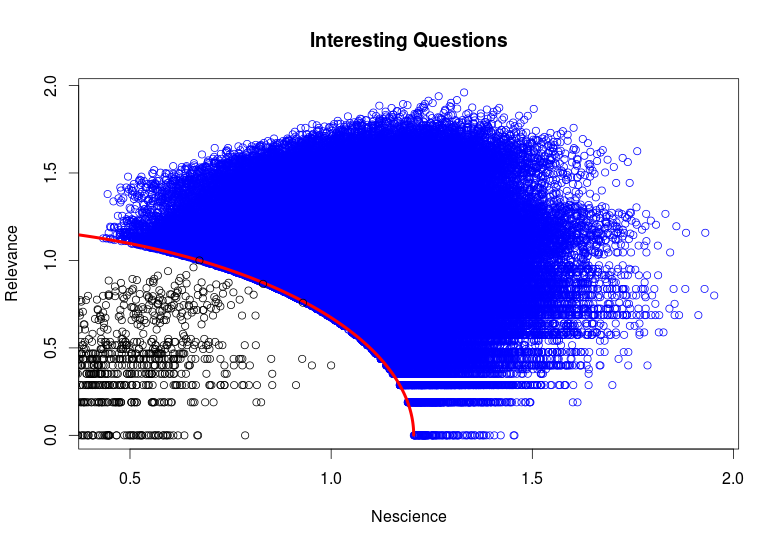
\includegraphics[scale=0.5]{NewQuestions}
\caption{\label{fig:Interesting-Intradisciplinary-Qu}Interesting Intradisciplinary
Questions}
\end{figure}

Table \ref{tab:Serendipity-Topics} contains a list of the top 25
candidates to become new topics topics according to their interestingness.
In this analysis we have included all the topics from all the knowledge
areas. Most of the questions deal with the concept of intellectual
property (\emph{copyright}, \emph{open access}, \emph{public domain},
and perhaps, \emph{wiki}), suggesting that this is an area where there
are still a lot of things to discover, much more that we are aware
of. Perhaps, it could be also a problem of a certain bias of Wikipedia
to these, and related, topics. Further investigation is required to
clarify this point.

In order to understand how new topics are generated, we have selected
the following two examples:
\begin{itemize}
\item New topic 17: \emph{Public domain + Earth}. This question rises the
issue if the Earth should be considered as a public resource; it touches
the very concept of private property. The methodology suggest that
this is not a very well understood topic.
\item New topic 18: \emph{Public domain + Internet}. Raises the same issue
that Question 17, but in this case restricted to Internet and its
governance.
\end{itemize}
Unfortunately, in both cases we fail to provide a well defined, innovative,
and previously unseen, research topic.

\begin{table*}
\begin{centering}
\begin{tabular}{|l|c|c|}
\hline 
{Problem} & Problem & Interestingness\tabularnewline
\hline 
\hline 
Public domain & Open access & 1.71\tabularnewline
\hline 
{Public domain} & REST & 1.70\tabularnewline
\hline 
Public domain & Wiki & 1.70\tabularnewline
\hline 
Open access & REST & 1.70\tabularnewline
\hline 
Copyright & Public domain & 1.69\tabularnewline
\hline 
Open access & Wiki & 1.69\tabularnewline
\hline 
Public domain & QR code & 1.69\tabularnewline
\hline 
Copyright & Open access & 1.68\tabularnewline
\hline 
Wiki & REST & 1.68\tabularnewline
\hline 
Open access & QR code & 1.68\tabularnewline
\hline 
Public domain & Transport Layer Security & 1.68\tabularnewline
\hline 
Copyright & REST & 1.68\tabularnewline
\hline 
QR code & REST & 1.67\tabularnewline
\hline 
Open access & Transport Layer Security & 1.67\tabularnewline
\hline 
Copyright & Wiki & 1.67\tabularnewline
\hline 
Wiki & QR code & 1.67\tabularnewline
\hline 
Public domain & Earth & 1.67\tabularnewline
\hline 
Public domain & Internet & 1.67\tabularnewline
\hline 
REST & Transport Layer Security & 1.66\tabularnewline
\hline 
Copyright & QR code & 1.66\tabularnewline
\hline 
Earth & Open access & 1.66\tabularnewline
\hline 
Internet & Open access & 1.66\tabularnewline
\hline 
Public domain & Open source & 1.66\tabularnewline
\hline 
Public domain & Web 2.0 & 1.66\tabularnewline
\hline 
Wiki & Transport Layer Security & 1.66\tabularnewline
\hline 
\end{tabular}
\par\end{centering}

\caption{\label{tab:Serendipity-Topics}New Topics}
\end{table*}


We could also restrict our search of new topics to a reduced number
of knowledge categories. For example, in Table \ref{tab:Restricted-Serendipity}
contains the ten most interesting new topics corresponding to the
already studied areas of \emph{theory of computation} and a new area
of \emph{phenomenology} (from Level 2 \emph{philosophy of mind}, and
Level 1 \emph{cognitive science}). Given the list of topics contained
in the table, we could come up with, for example, the following potential
new topics:
\begin{itemize}
\item New topic 2:\emph{ Turing machine} + \emph{synesthesia}: this new
topic could be about a new kind of Turing machine that incorporates
synesthesic properties. These new s\emph{ynesthesic Turing machines}
could be defined as the union of a group of Turing machines that are
linked together in such a way that when one machines read a symbol
from its tape, it produces an automatic change in the state of another
machine. The property of synesthesia could be also extended to the
case of non-deterministic Turing machines.
\item New topic 4:\emph{ Kolmogorov Complexity} + \emph{Self-awarenes}:
This topic could be interpreted as investigating the minimum complexity
required for a computer program to have the capacity of self-awareness.
\end{itemize}
\begin{table*}
\begin{centering}
\begin{tabular}{|l|c|c|}
\hline 
{Question} & Question & Interestingness\tabularnewline
\hline 
\hline 
Kolmogorov complexity & Change blindness & 1.24\tabularnewline
\hline 
{Turing machine} & Synesthesia & 1.23\tabularnewline
\hline 
Kolmogorov complexity & Qualia & 1.23\tabularnewline
\hline 
Kolmogorov complexity & Self-awareness & 1.22\tabularnewline
\hline 
Turing machine & Qualia & 1.22\tabularnewline
\hline 
Kolmogorov complexity & Synesthesia & 1.21\tabularnewline
\hline 
Turing completeness & Synesthesia & 1.20\tabularnewline
\hline 
Turing machine & Self-awareness & 1.20\tabularnewline
\hline 
Turing completeness & Qualia & 1.20\tabularnewline
\hline 
Turing completeness & Self-awareness & 1.18\tabularnewline
\hline 
\end{tabular}
\par\end{centering}

\caption{\label{tab:Restricted-Serendipity}Restricted New Topics}
\end{table*}

%
% Section: Philosophy of Science
%

\section{Philosophy of Science}

Philosophy of science is a branch of philosophy concerned with the foundations and methods of science. The central issues addressed by the philosophers of science are the following:

\vskip 0.25cm

\begin{itemize}
\item Does science allow us to reach an absolute knowledge?
\item What are scientific theories? How do we evaluate competing theories?
\item How are theories discovered and evaluated? Is there a universal scientific method?
\item What is scientific explanation? What it is problem solving? Does science enable progress?
\item What it is the difference between science and pseudosicence?
\end{itemize}

\vskip 0.25cm

Unfortunately, up to today there is no consensus among philosophers about the right answers. Although the theory of nescience has not been explicitly designed to provide a solution to any of these open problems, since it is a theory to be applied in practice, not a framework to understand how we gather knowledge or to explain what science is, we think we could provide a possible interpretation that might bring some light into these fundamental questions. In the next paragraphs we provide a short summary of how these inquiries about science itself could be addressed in the context the theory of nescience, and the rest of the chapter provides the details of the answers that the theory of nescience provides.

\vskip 0.5cm

% Q: Does science allow us to reach an absolute knowledge?

\emph{Q: Does science allow us to reach an absolute knowledge?}

Philosophers of science deal with the problem of how knowledge about our world is gathered trough our senses, and if we can trust our perceptions. Also, they address the difficult issue of how knowledge is derived from facts (for example, by means of applying the principle of induction), and if it is sound, from a logic point of view, to make those derivations. Finally, philosophers are interested in how scientific theories are generated based in this knowledge. Any of these problems is covered by the theory of nescience, since we assume that theories (or descriptions in our own terminology) are already known. We do not provide any method to create those theories. What the theory of nescience provides is a set of metrics to quantitatively evaluate, and compare, existing scientific theories. 

It might appear that the descriptions in which the theory of nescience is based are truly objective, in the sense that they must be so clear and well stated that even a computer can reconstruct the original topic given its description. Although this point is true, the problem that prevents the theory to provide an absolute knowledge about our world is the way we choose the entities to study, and how we encode as strings those entities. As we have seen (see Chapter \ref{cha:Topics-and-Descriptions}), the accuracy of our descriptions depend on how good is our encoding of the abstract entities we are studying. Unless the entities are strings themselves, we must assume that our encoding could not be perfect. Moreover, we could be wrong about our assumption that the selected set of entities covers all possible entities of that kind. That is, the set of entities are subject to change as our scientific understanding about them develops. {\color{red} The same might happen in case of encodings.}

Although the theory of nescience does not say anything about how we can reach an absolute knowledge about an entity, it can tell us if we have reached a perfect description (that we make equal to a perfect knowledge). That is, the theory of nescience can answer the question if we have reached a perfect knowledge about a topic, subject that the the entity under study has been properly identified, and the encoding of this entity has no errors.

\vskip 0.5cm

% Q: How do we evaluate competing scientific theories?

\emph{Q: How do we evaluate competing scientific theories?}

There exists multiple methods for the comparison of competing scientific theories. Karl Popper's falsificationism is a well known one. According to Popper, scientific theories must be falsifiable, that is, they must be so clearly stated and precise that we can validate them by means of performing an experiment. The more precisely a theory is formulated, and the more accurate its predictions, the better, since that increases the chances of being falsified. As long as the experiments confirm the theory we keep it as valid. However, if a single experiment fails, the theory should be rejected. The main problem of falsificationism is that, in practice, if a experiment fails to confirm a theory, we can not be sure about what went wrong, the experiment or the theory. In the theory of nescience we completely agree with Popper's idea that theories must be clearly stated. In fact, our theories, being Turing machines, are as clearly stated as possible. But, on the contrary of what falsificationism proposes, we do not reject a theory because it has been falsified with an experiment, instead what we propose is to measure the error produced, and take that error into account in our measure of how good is the theory, that is, the nescience of our current best description. Another difference is that, in principle, a theory that makes better prediction is not automatically preferred to another one with less predictability, since we have to take into account not only the error, but also the redundancy of the theory. Unfortunately, in practice, the theory of nescience suffers the same problem than falsificationism, since given that the error of a description must be estimated in practice, usually by means of performing an experiment, we can not be sure if the error is due to the incorrectness of the theory, or due to a wrong designed experiment.

Other alternative interpretations of science, with a stronger orientation towards the theoretical frameworks in which scientific activities take place, like Kuhn's scientific paradigms or Lakatos' research programs, do not have a clear interpretation in the context of the theory of nescience. The same happens when we take into account the social or political aspects of science. Please mind that we are not saying that these possible explanations of science are incorrect. In fact, we have taken seriously the recommendations of Popper, Kuhn, Lakatos and many other philosophers of science during the development of our own theory of nescience.

\vskip 0.5cm

% Q: Is there a universal scientific method?

\emph{Q: Is there a universal scientific method?}

Although we provide a methodology for the discover of interesting questions, a method to discover what it is hidden in the unknown area, the theory of nescience does not, and does not intend, to be a method (or methodology) for the development of new science. However, in the framework provided by the theory of nescience we could address the problem of which one of the scientific methods proposed so far is more effective to discover new theories. By means of an historical analysis, and by means of analyzing how well the evolution of error and redundancy is covered by the method.

{\color{red} TODO: How non-falsifiable theories are managed by the theory of nescience? What about the desirable property of being as much falsifiable as possible?}

Nescience provides a tool that can be applied to all disciplines. 

Feyerabend aregues that there is no such method, he proposes the principle that "anything goes". anarchistic account of science [...] "increases the freedom of scientists by removing them from methodological constraints"

\vskip 0.5cm

% Q: Does science enable progress?

\emph{Q: Does science enable progress?}

{\color{red} TODO: Generality of a theory (the amount of things it can exlain), and the problem of too generic theories. Is there somethin like "information content" of a theory}

Popper sugested to propose highly speculative, hihgly falsifiable, theories. That it is in line with our methodology to the discovery of new research topics. According to Popper we cannot say that a theory is true, just that it is the best, yet non falsified, theory. New theories must be more falsifiable than the ones they replace. An ad-hoc modification that does not decreases the error, will increase the nescience because it increases the redundancy. However, to Popper, a prediction is novel if it involves a phenomenon that does not figure in the background knowledge of the time.


"According to Kuhn, science progress following the following schema: pre-science, normal science, crisis, revolution, new normal science, new crisis [...] There will be no purely logical argument that demonstrates the superiority of one paradigm over another and that thereby compels a rational scientist to make the change [...] proponents of rival paradigms will subscribe to different sets of standars and metaphysical principles [...] rival paradigms are incommensurable."

\vskip 0.5cm

% Q: What it is the difference between science and pseudosicence?

\emph{Q: What it is the difference between science and pseudosicence?}

As it was pointed out by Feyerabend, all the different proposals made by philosophers to identify that remarkable method that makes science possible (logical positivist, falsificationism, theory-dependent models, etc.) failed even to explain a classical example like the Copernican revolution. According to Feyerabend, there is no such thing as a scientific method; instead, he proposed that in science, anything goes. Moreover, Feyerabend asserts that there is nothing special about science that makes it superior to other forms of knowledge. We completely disagree with this anarchist point of view. As we will see in detail in Section \ref{sec:evolution-knowlege}, the theory of nescience provides a clear answer to the question of what distinguishes science from pseudoscience. According to our theory, in science we have that nescience decreases when we invest an amount of effort to gather new knowledge, however, in pseudosciences, nescience does not decreases in spite of the effort invested.

Unfortunately, this capacity of decrease nescience given effort is a necessary condition to classify a knowledge discipline as scientific, but not a sufficient one. That is, not all disciplines in which nescience decreases with effort are classified as science according to our intuitive idea of what it is science. For example, {\color{red} XXX} is a case of a discipline in which nescience decreases with time but it is not considered to be a science.

%
% Section: Evolution of Knowledge
%

\section{Evolution of Knowledge}
\label{sec:evolution-knowlege}

{\color{red} TODO: Show the evolution of a research topic, preferably by using historical data from centuries ago, if not possible, using the evolution of a tipic given wikipedia.}

\begin{example}
In Figure \ref{fig:TheoreticalPerfectKnowledge} is depicted the evolution of a hypothetical research topic. Every point in the graph represents a new current best description for that topic (descriptions are ordered with respect to time). New descriptions could be based on novel theories that explain the topic, refinements over already existing ones, or on a reduction of the number of assumptions. In general, each new description should be shorter than the previous one. However, as we can see in the figure, it might happen that some descriptions are longer than its previous. That could be the case, for example, when we discover new facts that have to be taken into account by the theory. But the important thing is that nescience should decrease, in average, with time.
\end{example}

\begin{figure}[h]
\centering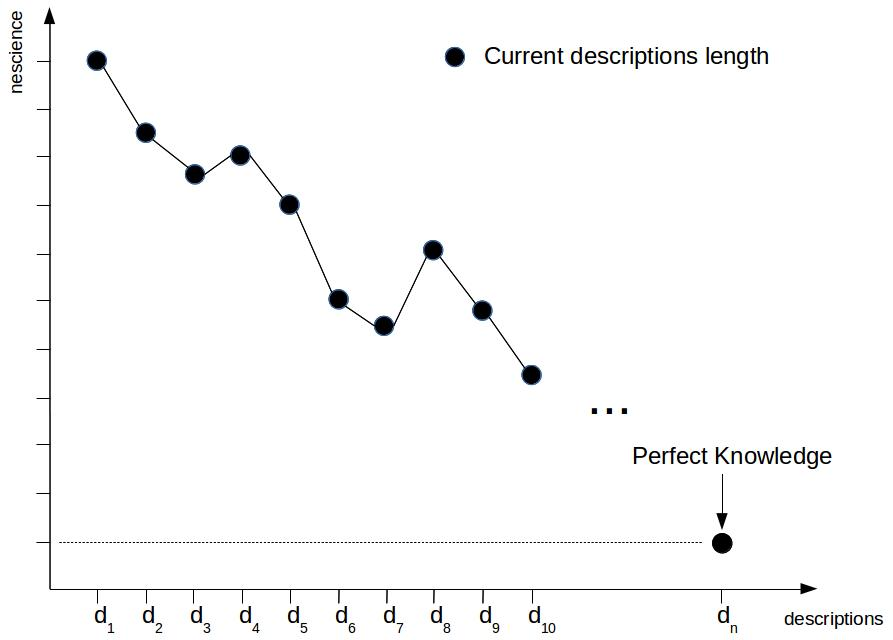
\includegraphics[scale=0.5]{TheoreticalPerfectKnowledge}
\caption{\label{fig:TheoreticalPerfectKnowledge}Evolution of Nescience}
\end{figure}


My hypothesis is that the nescience of topic descriptions decrease with time. On the contrary, the description of topics from pseudocience or religion does not decrease with time. This property, decrease with time is what distinguish science with respect other pseudosiences. I totally disagree with Feyerabend when he states that \emph{sicence has no special features that render it intrinsically superior to other kinds of knowledge such as ancient myths or voodoo}.

How does my view differ with respect to the point of view that states that "science is derived from facts"? Perhaps facts is what allow us to make shorter descriptions. But facts also can increase the length of a description.

Here I have to be very careful, becase if the description lenght of topics in phylosophy does not decrease with time, we should conclude that phylosophy is a pseudocience.

In order to understand a theory a background knowledge is assumed. What it is exactly that background is something that depends on the theory and the current undertanding of the theory.

\begin{example}
Suppose that the topic $t$ being studied is the concept of \emph{limit
of a function}. The standard \emph{$\left(\epsilon,\delta\right)$-definition
}of limit provided by Karl Weierstrass is:

\begin{eqnarray*}
\lim_{x\rightarrow c}f(x) & = & L\Leftrightarrow\forall\epsilon>0\:\exists\,\delta>0\,:\,\\
 &  & \forall x\,\left(0<\left|x-c\right|<\delta\Rightarrow\left|f(x)-L\right|<\epsilon\right)
\end{eqnarray*}


This definition has a length of 46 symbols, spaces not included%
\footnote{\begin{example}
For the sake of simplicity, we have computed the complexity of the
topic given the number of symbols, not the the length of its binary
representation, as it is required by our definition.\end{example}
%
}. The alternative \emph{infinitesimal definition} of limit, based
on non-standard calculus, is:

\[
\lim_{x\rightarrow c}f(x)=L\Leftrightarrow st(x)=c\Rightarrow st(f(x))=L
\]


where $st(\cdot)$ denotes the \emph{standard part function}, which
\textquotedbl{}rounds off\textquotedbl{} each finite hyperreal%
\footnote{Nonstandard analysis deals primarily with the pair $\mathbb{R\subset^{\star}\mathbb{R}}$,
where hyperreals $^{\star}\mathbb{R}$ are an ordered field extension
of the reals $\mathbb{R}$, that contains infinitesimals in addition
to reals.%
} number to the nearest real. This second definition has a length of
31 symbols, and so, we say that our nescience of the concept of limit
has decreased, since we were able to simplify the definition from
a three quantifier block to a just one quantifier statement.

If the complexity $C_{t}$ of the concept of limit is less that 31
characters, then there must be possible to come up with a even shorter
definition.\hfill{}$\square$
\end{example}

%
% Section: Graspness of Topics
%

\section{Graspness of Topics}

In Section {\color{red} ref?} we saw a masure of how difficult is to grasp a research area. In this section we are going to see a measure of how difficult is to grap a individual research topic.

{\color{red} TODO: Study the graspness of a research topic difficult to understand, and the graspness of a easy to understand topic}

%
% Section: Probability of Being True
%

\section{Probability of Being True}

{\color{red} TODO: Study the probability of being true.}

{\color{red} TODO: If the acceptability of experimental results is theory-dependent, how can we change the probability of being true of a theory in the presense of new experimental results? There is a high risk of circular argument in the bayesian interpretation of science.}

The Bayesian interpretation of science, based on the Bayes theorem of conditional probabilities, states that the probability that an hypothesis $H$ is true given that an experiment $E$ has been sucessfull, $P(H|E)$, is given by:
\[
P(H|E) = P(H) \frac{ P(E|H) }{ P(E) }
\]
where $P(H)$ is the prior probability of $H$, $P(E|H)$ is the probability of being the experiment sucessfull given that the hypothesis is true, and $P(E)$ is the probability of being true the experiment. In this way, Bayes is a continuous proces in which every sucessfull experiment will increase the probability of $H$ being true, and a failed experiment ({\color{red} How?}) will decrease the probability. The very initian probability $P(H)$, prior to any experiment, is given by the length of its description:
\[
P(H) = r^{l(H)}
\]

\begin{example}
{\color{red} TODO: A real example, with data}
\end{example}

{\color{red} TODO: How my theory of nescience integrates with this?}

{\color{red} TODO: How the base knowledge $a$ affect the probability of the hypothesis $H$?}

{\color{red} TODO: How can we use Bayes and what-if scenaries to improve an hypothesis?}

\section{Unused text}

Here I should mention the work of Solomonof with respect to assign a prior probability to theories. I what Solomonof proposed was to use the shortest lenght of programs, what I propose is essentially different, since what I use is lengths of descriptions.

The same that we do not try to define what it is a research topic, I do not try to provide an explanation of from where scientific theories come from. According to my interpretation, anything could be a theory, with a initial probability of being true. However, we, as scientists, could clean-up those very unlikely of being true theories.

I will show that the distinctive element of scientific knowledge is that with time nescience decreases, as opposed to other kinds of knowlege, such as ancient myths or voodoo, where nescience does not decrease with time.

Scientific knowledge can neither be consclusively proved nor conclusively disproved, but we can assign a probability of being true, a probability that will change with time, as new facts are discovered, and new experimetns are performed.

Theories are based on the observation of facts and experimentation. Both, the observation of facts and the experiment desing are based on our current knowledge. If we have a defective knowledge, our theories would be defective. New knowledge, or new technologies, allows us to gather new facts, design new experiments, and define new theories.

Current theories will be eventually replaced in the future by new ones.

Theories are based on other theories and relate to other theories, forming a complex network of interrelations between theories.


%
% Section: References
%

\section*{References}


The behavior of compressors depending of the size of objects and window (buffer) size is studied in detail in \cite{cebrian2005common} with applications to the normalized compression distance (a measure of similarity between objects proposed in \cite{li2004similarity}).


